\documentclass[11pt]{scrartcl}

\usepackage{hyperref}
\usepackage{graphicx}

\title{CS104 Project Report}
\author{Bhavya Tiwari\thanks{Roll number \textsc{24B0913}}}

\begin{document}
\maketitle
\begin{abstract}
  This project report is in partial fulfilment of \textsc{CS104} course requirements,
  and details the structure of my project including packages used, design of
  the application and what all new things I learnt while attempting the problem
  statement. I have tried my best to make this enjoyable to read \texttt{:D}
\end{abstract}
\tableofcontents

\newpage

\section{Introduction}

In order to give us a feel of how larger code bases work, a project was assigned
to us in \textsc{CS104} which needed using multiple things that we had learnt
simultaneosly. It was a different experience from exam problems, where you start
afresh on a \emph{niche} problem suitable to attack by a particular tool (which
was mostly obvious after reading the problem statement); moreover, we had to
\emph{built up} on old code. It was quite an interesting experience.

\subsection{Choice of project}

For the project, we were given three options: making a log analysis website, or
a cricket live score website, or a simple angry birds style game. I chose to
make a log analysis website because its internal mechanics looked crystal clear
to me. It inherently looked quite modular (see \nameref{section:internals}) and
therefore easy to not mess up.

\subsection{Aim of the project}

To reiterate \cite{logfileprob}, this project aims to develop a Flask-based
(see \cite{flaskdocs}) web application that allows users to: 

\begin{itemize}
  \item Upload log files and convert them into structured CSV format.  
  \item Filter and sort logs to extract meaningful insights.
  \item Generate visualizations to interpret log data effectively.  
  \item Download processed logs and visualizations for further analysis.

\end{itemize}

\section{Using the Application}

To start the application execute the following command
and you will be greeted by the home page as in the figure.

\begin{verbatim}
  flask --app flaskwebsite_24b0913.py run
\end{verbatim}


\begin{figure}[htbp]
  
  \centering
  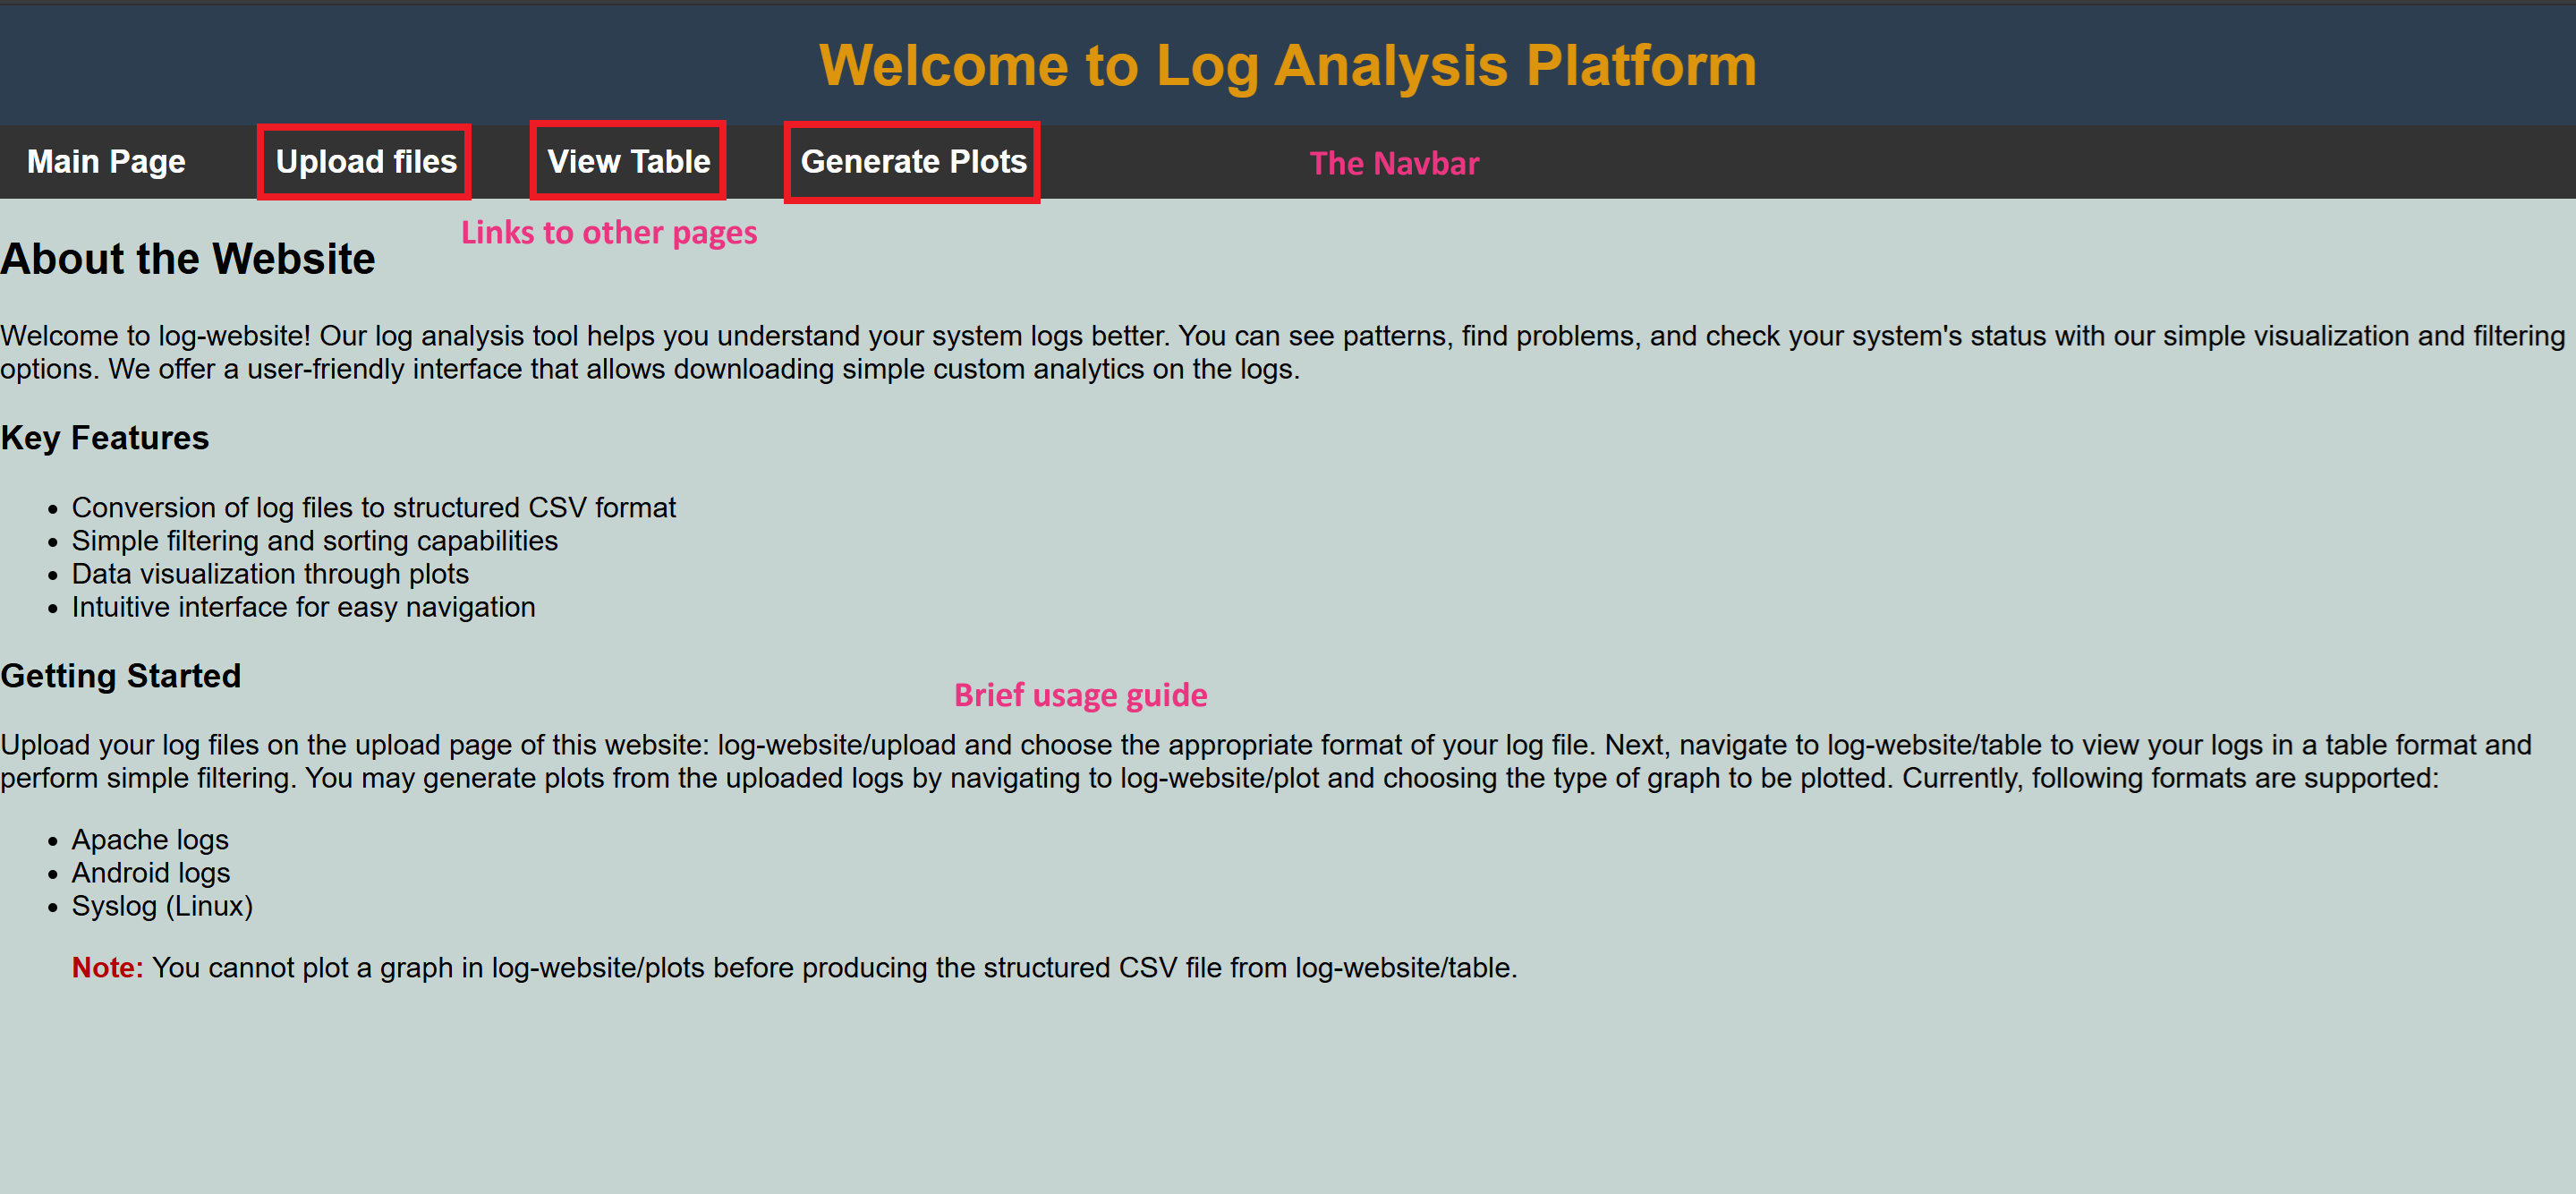
\includegraphics[width=\linewidth]{images/homepage.png}
  \caption{The home page of the website.}
  \label{homepage}

\end{figure}

To get started with log analysis, proceed to the upload page and upload your log
file using drag and drop interface (or a dialog box by clicking). All processing
is done \emph{lazily} except validation that is done instantly after the file is
received (see \nameref{philo}). Practically, this means that you can upload
multiple files one by one but you have to \emph{tell} the website which one do you
want to process first.



\begin{figure}[htbp]
  
  \centering
  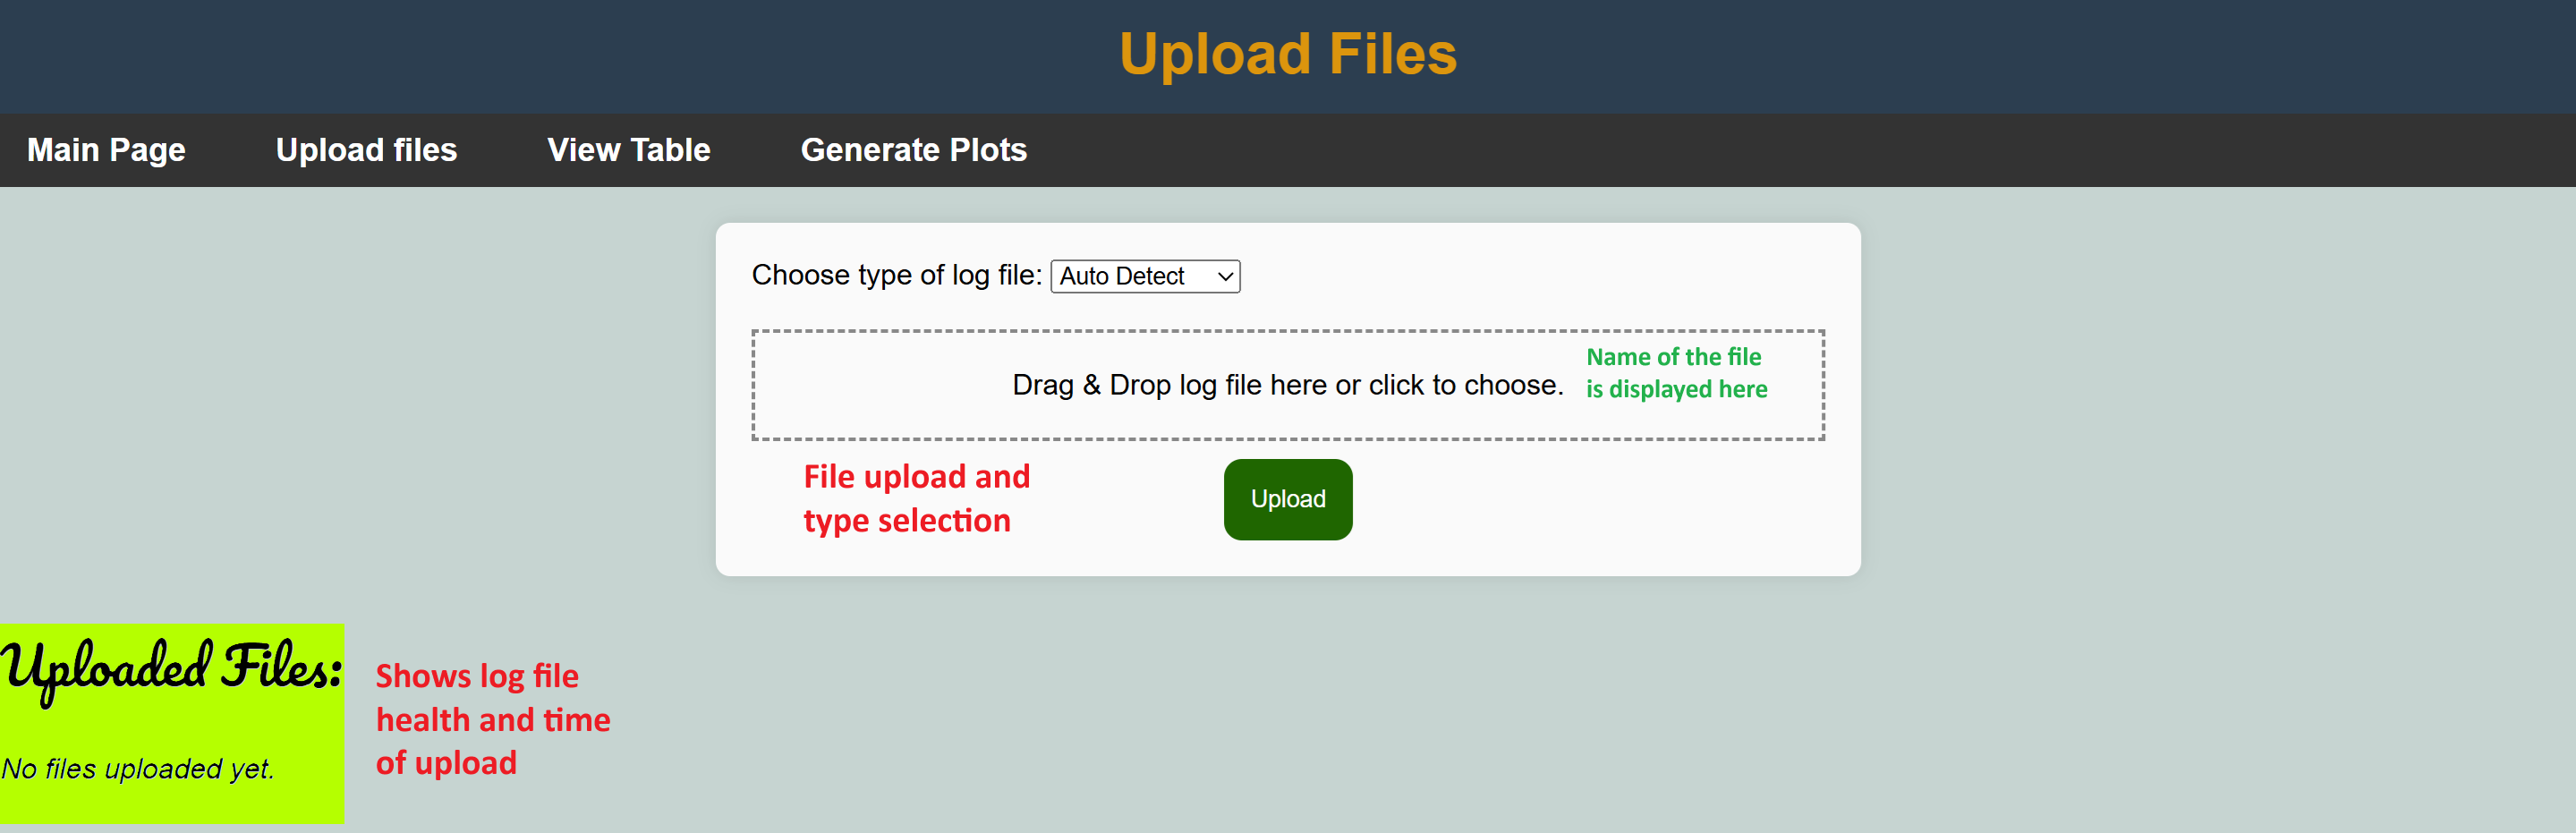
\includegraphics[width=\linewidth]{images/uploadpage.png}
  \caption{Form for uploading files on the upload page.}
  \label{uploadpage}

\end{figure}


\begin{figure}[htbp]
  
  \centering
  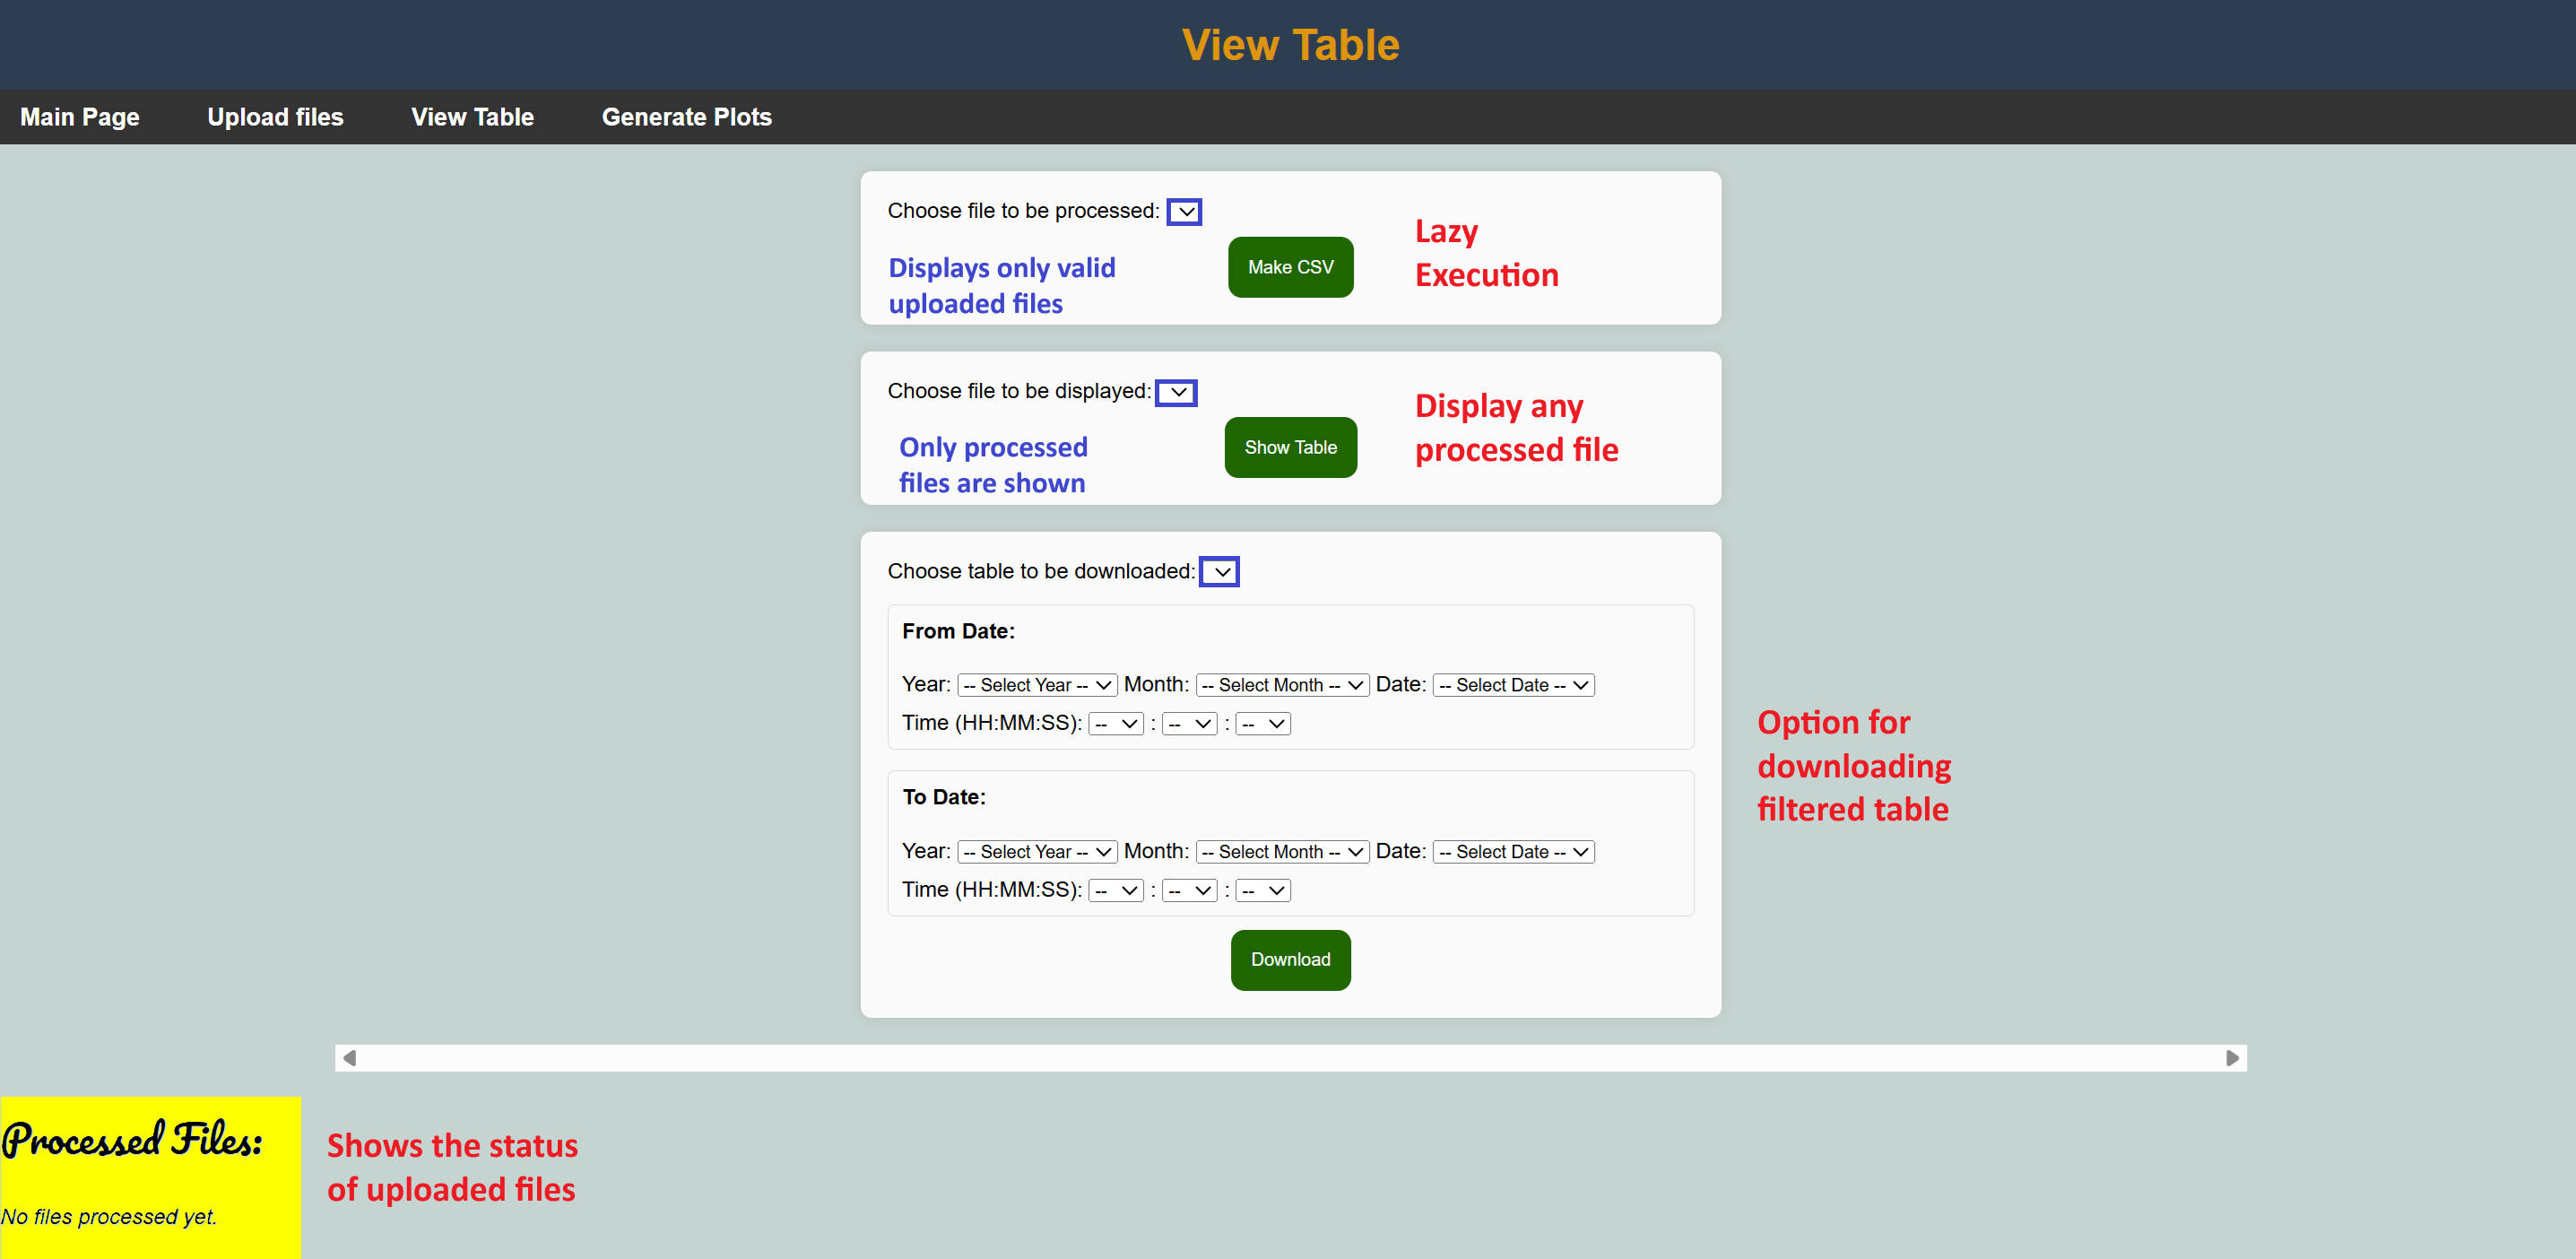
\includegraphics[width=\linewidth]{images/tablepage.png}
  \caption{Formatting the log file into a table.}
  \label{tablepage}

\end{figure}


\begin{figure}
  
  \centering
  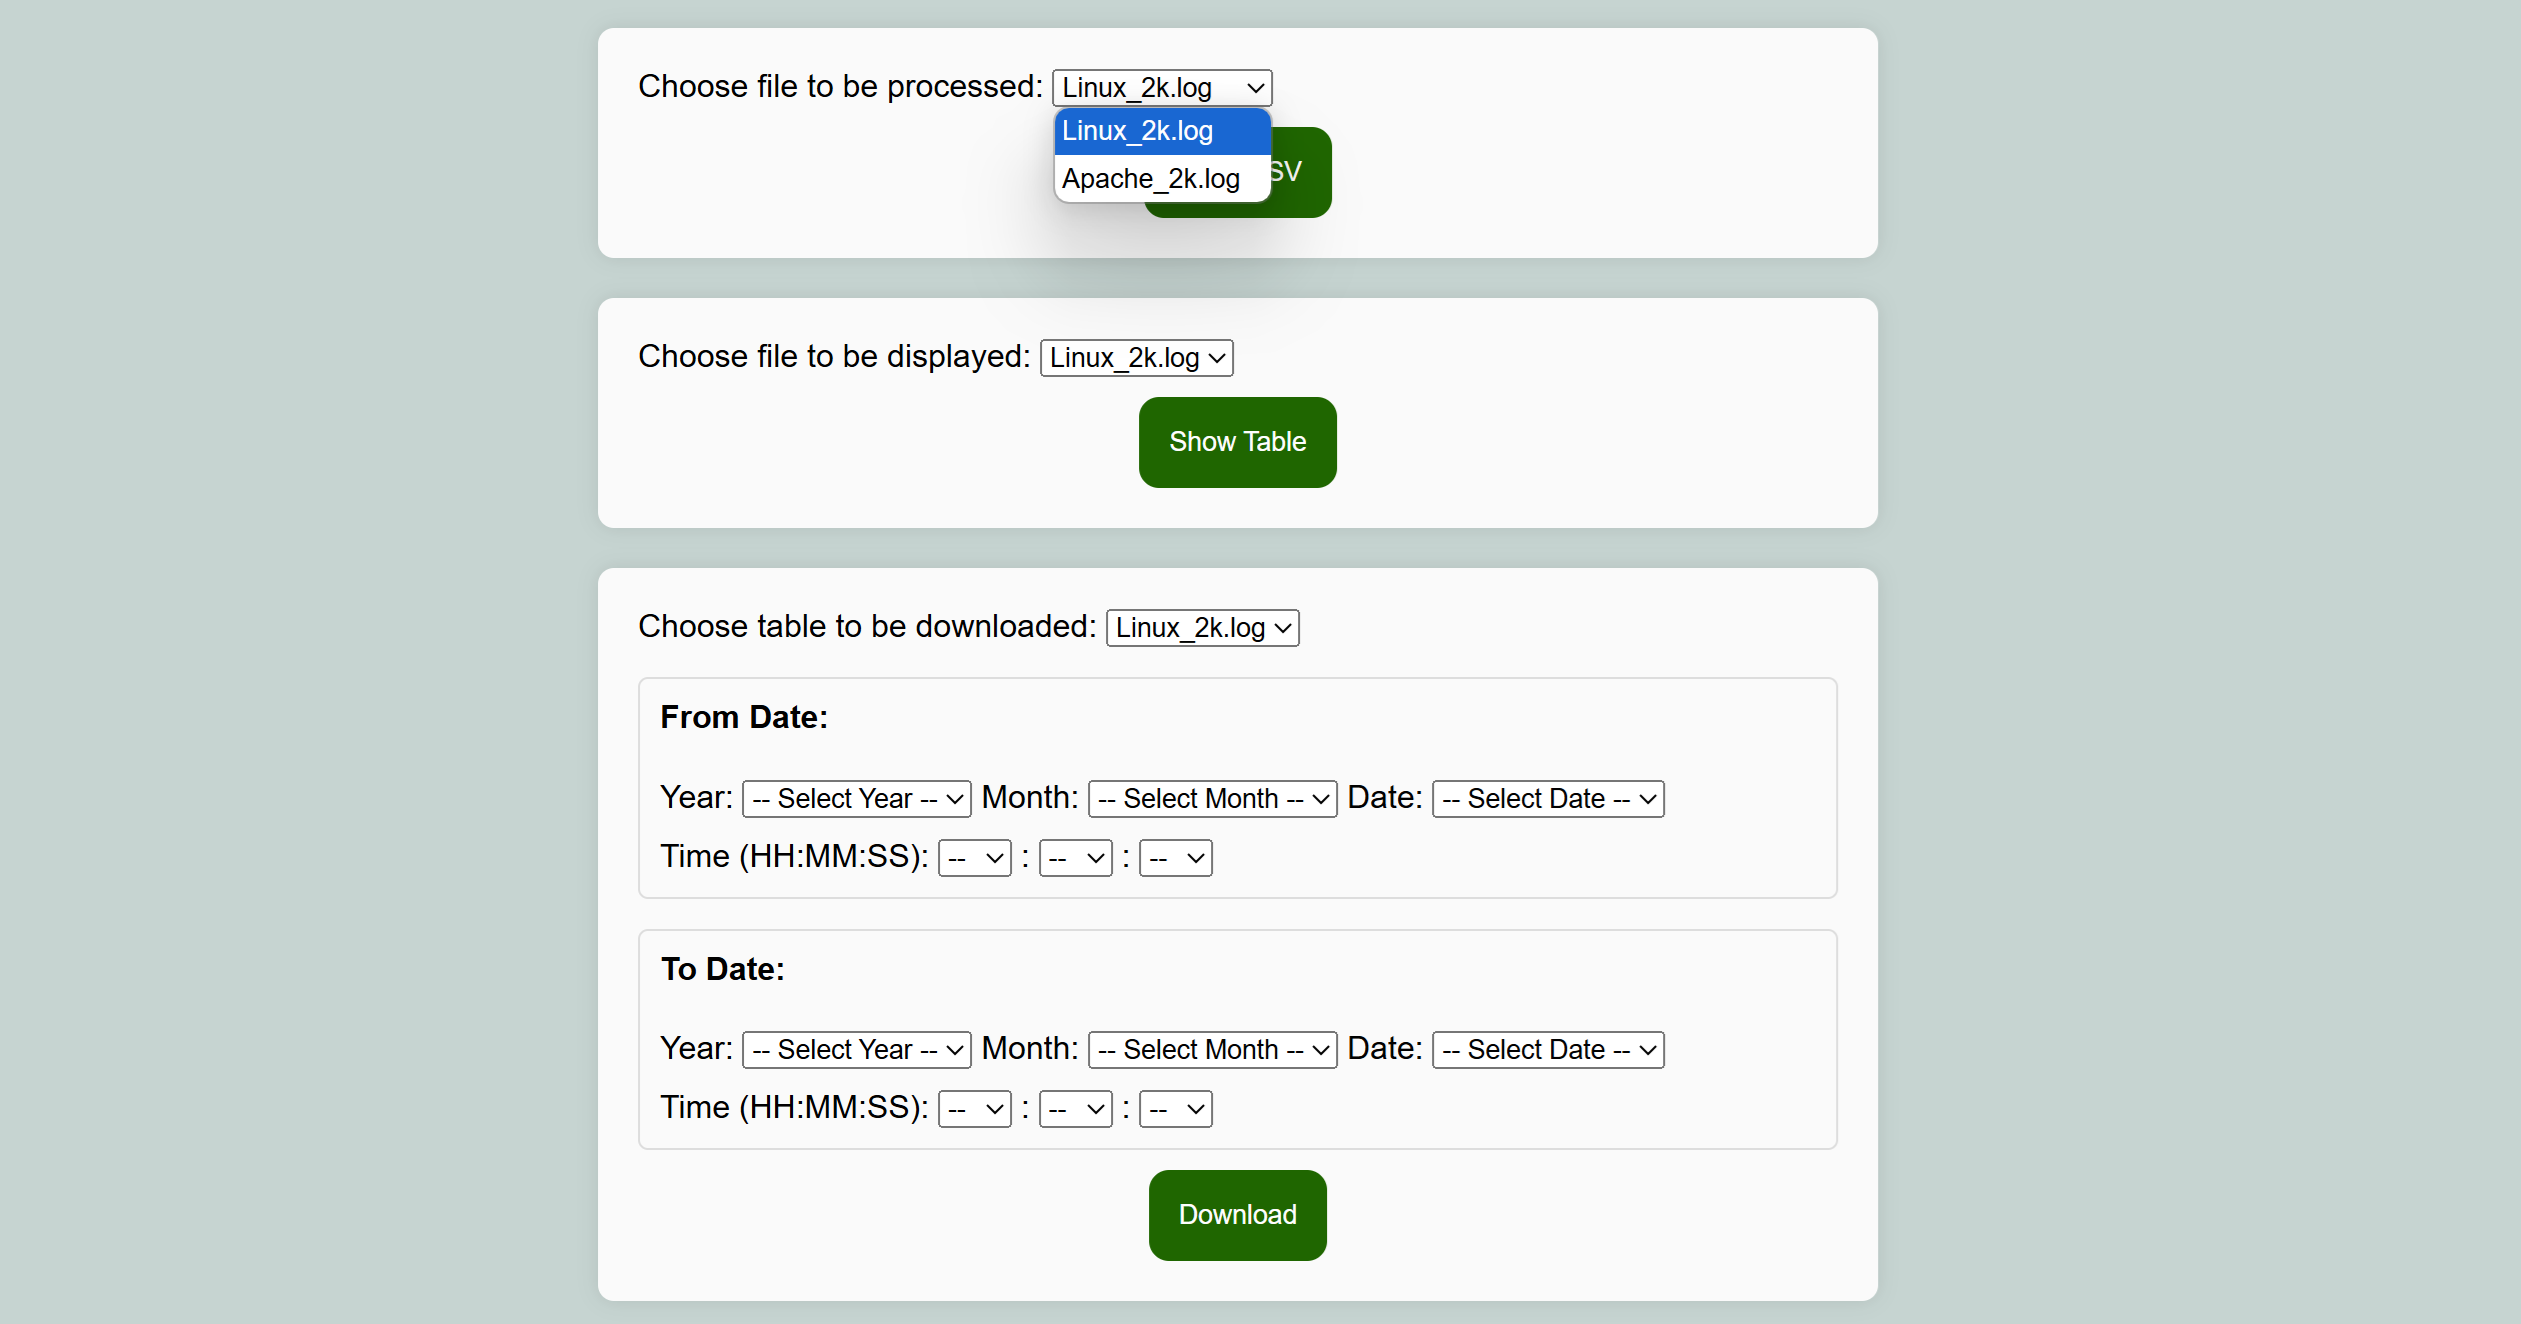
\includegraphics[width=\linewidth]{images/tableform.png}
  \caption{Valid files are shown in a drop down list.}
  \label{tableform}

\end{figure}



\begin{figure}
  
  \centering
  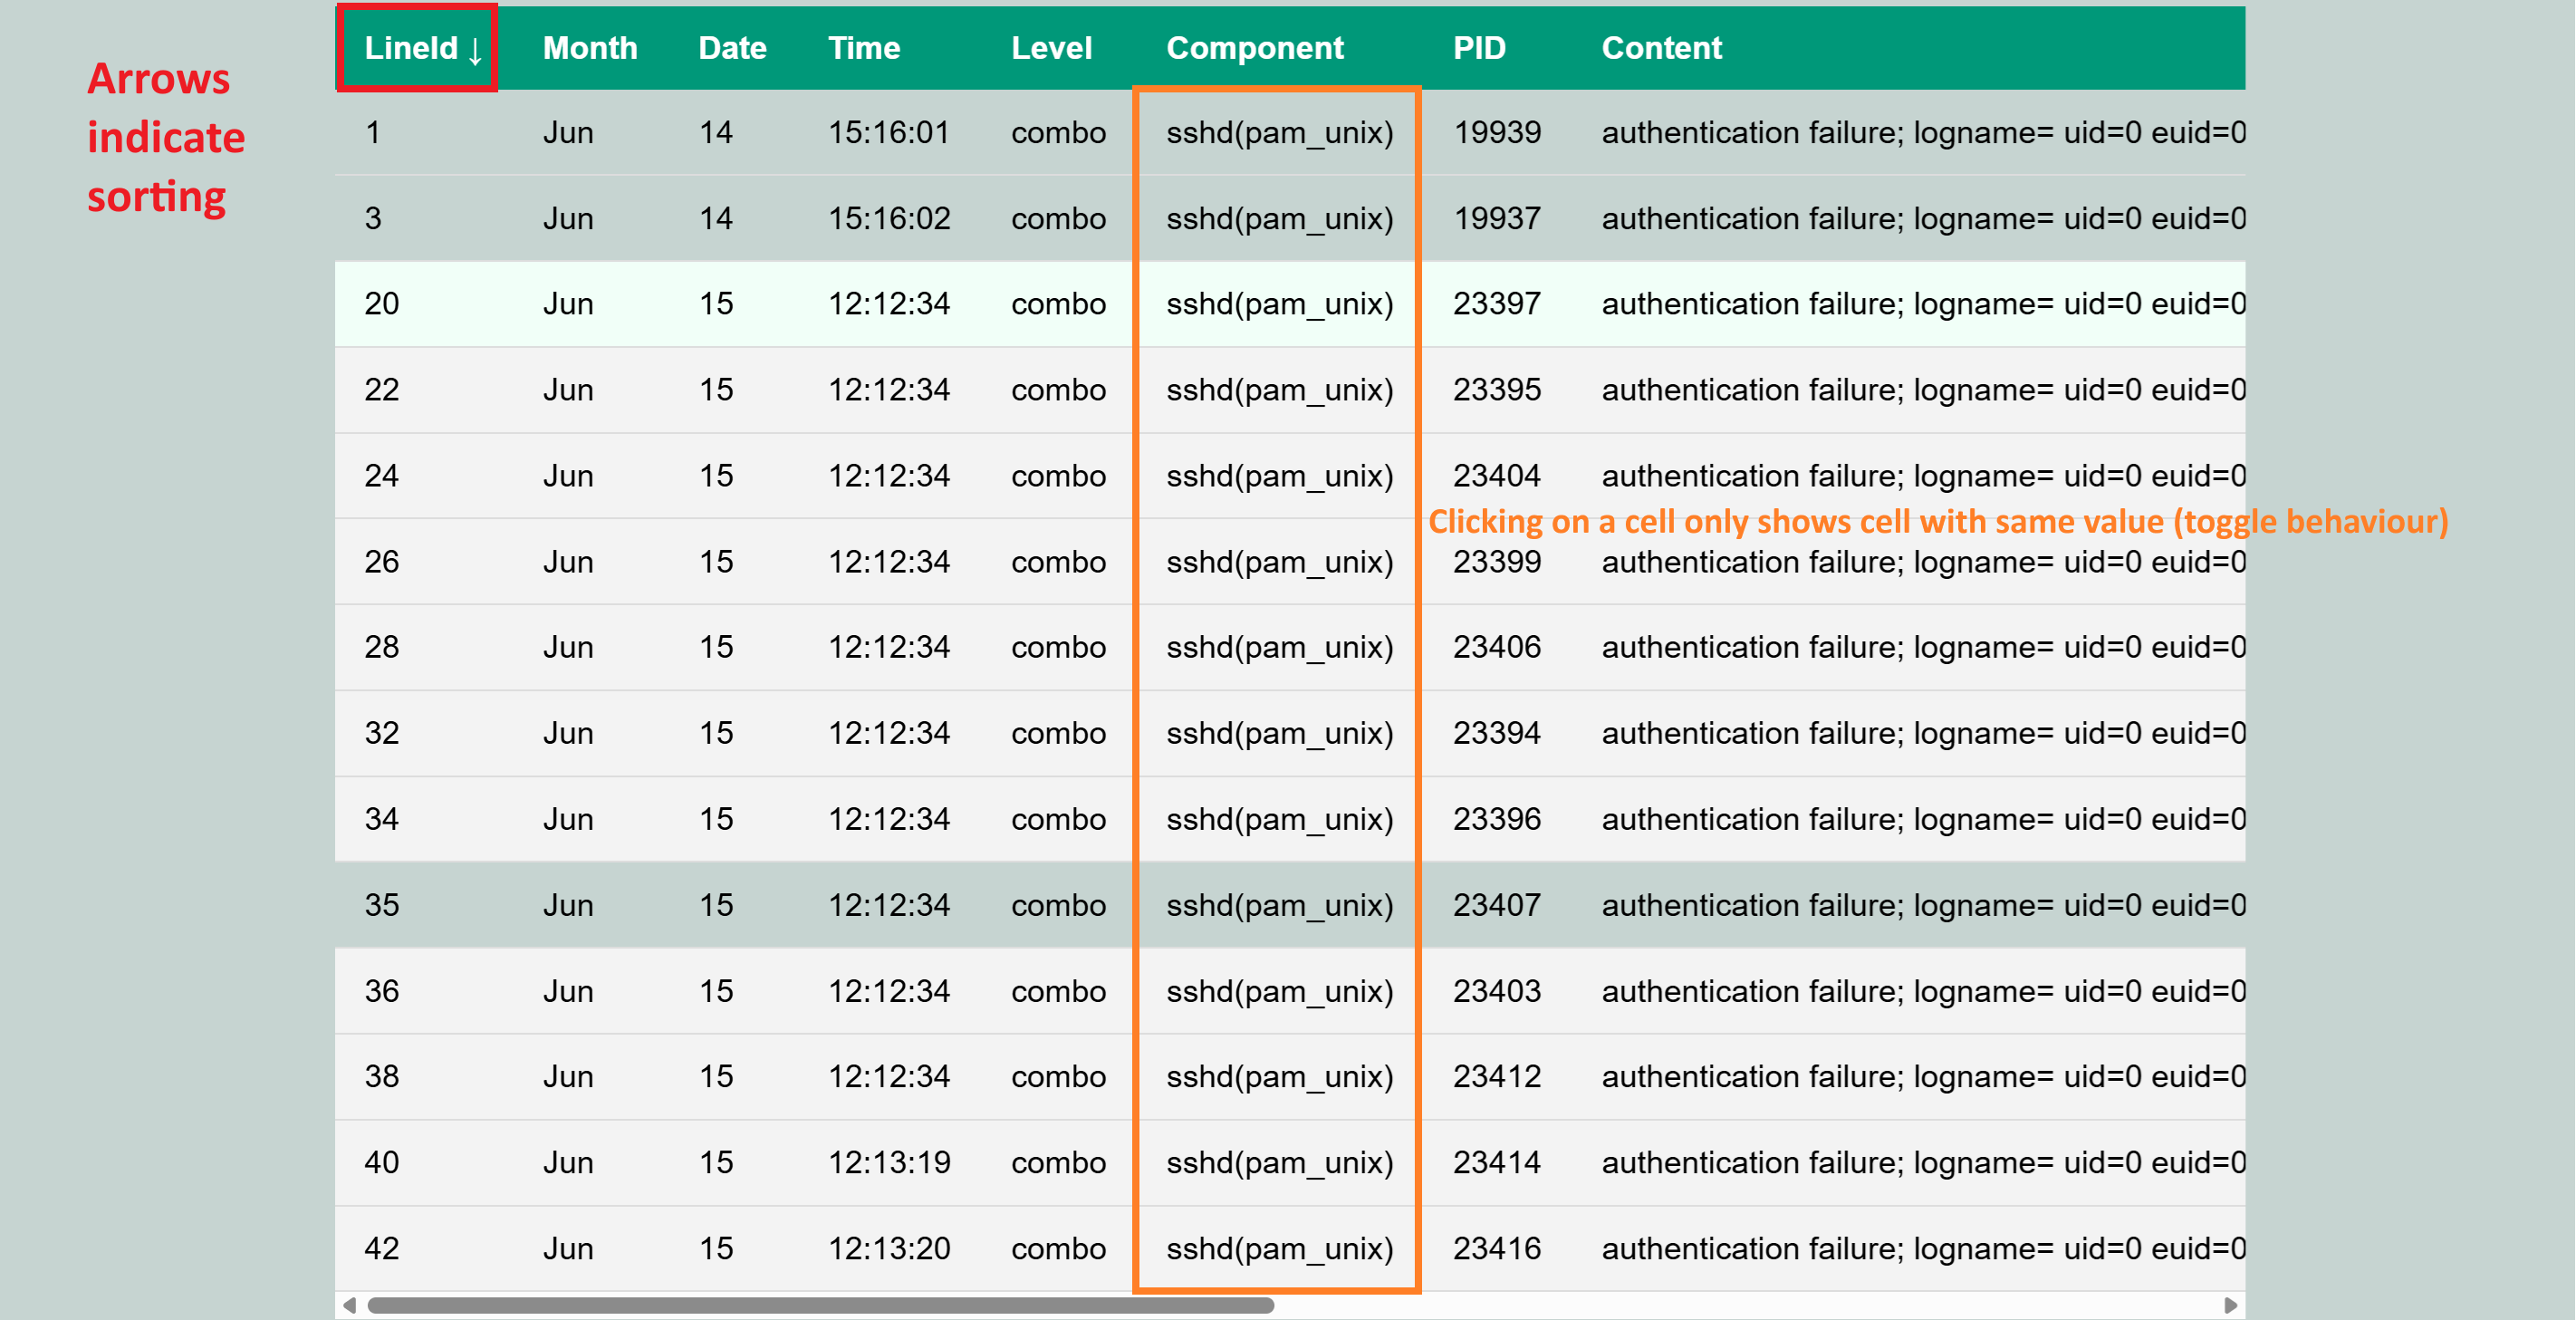
\includegraphics[width=\linewidth]{images/tableclick.png}
  \caption{Clicking on heading sorts the rows by value, while clicking on data
  cell only displays cells that have the same value in that column (as the
  clicked value).}
  \label{tableclick}

\end{figure}


\begin{figure}
  
  \centering
  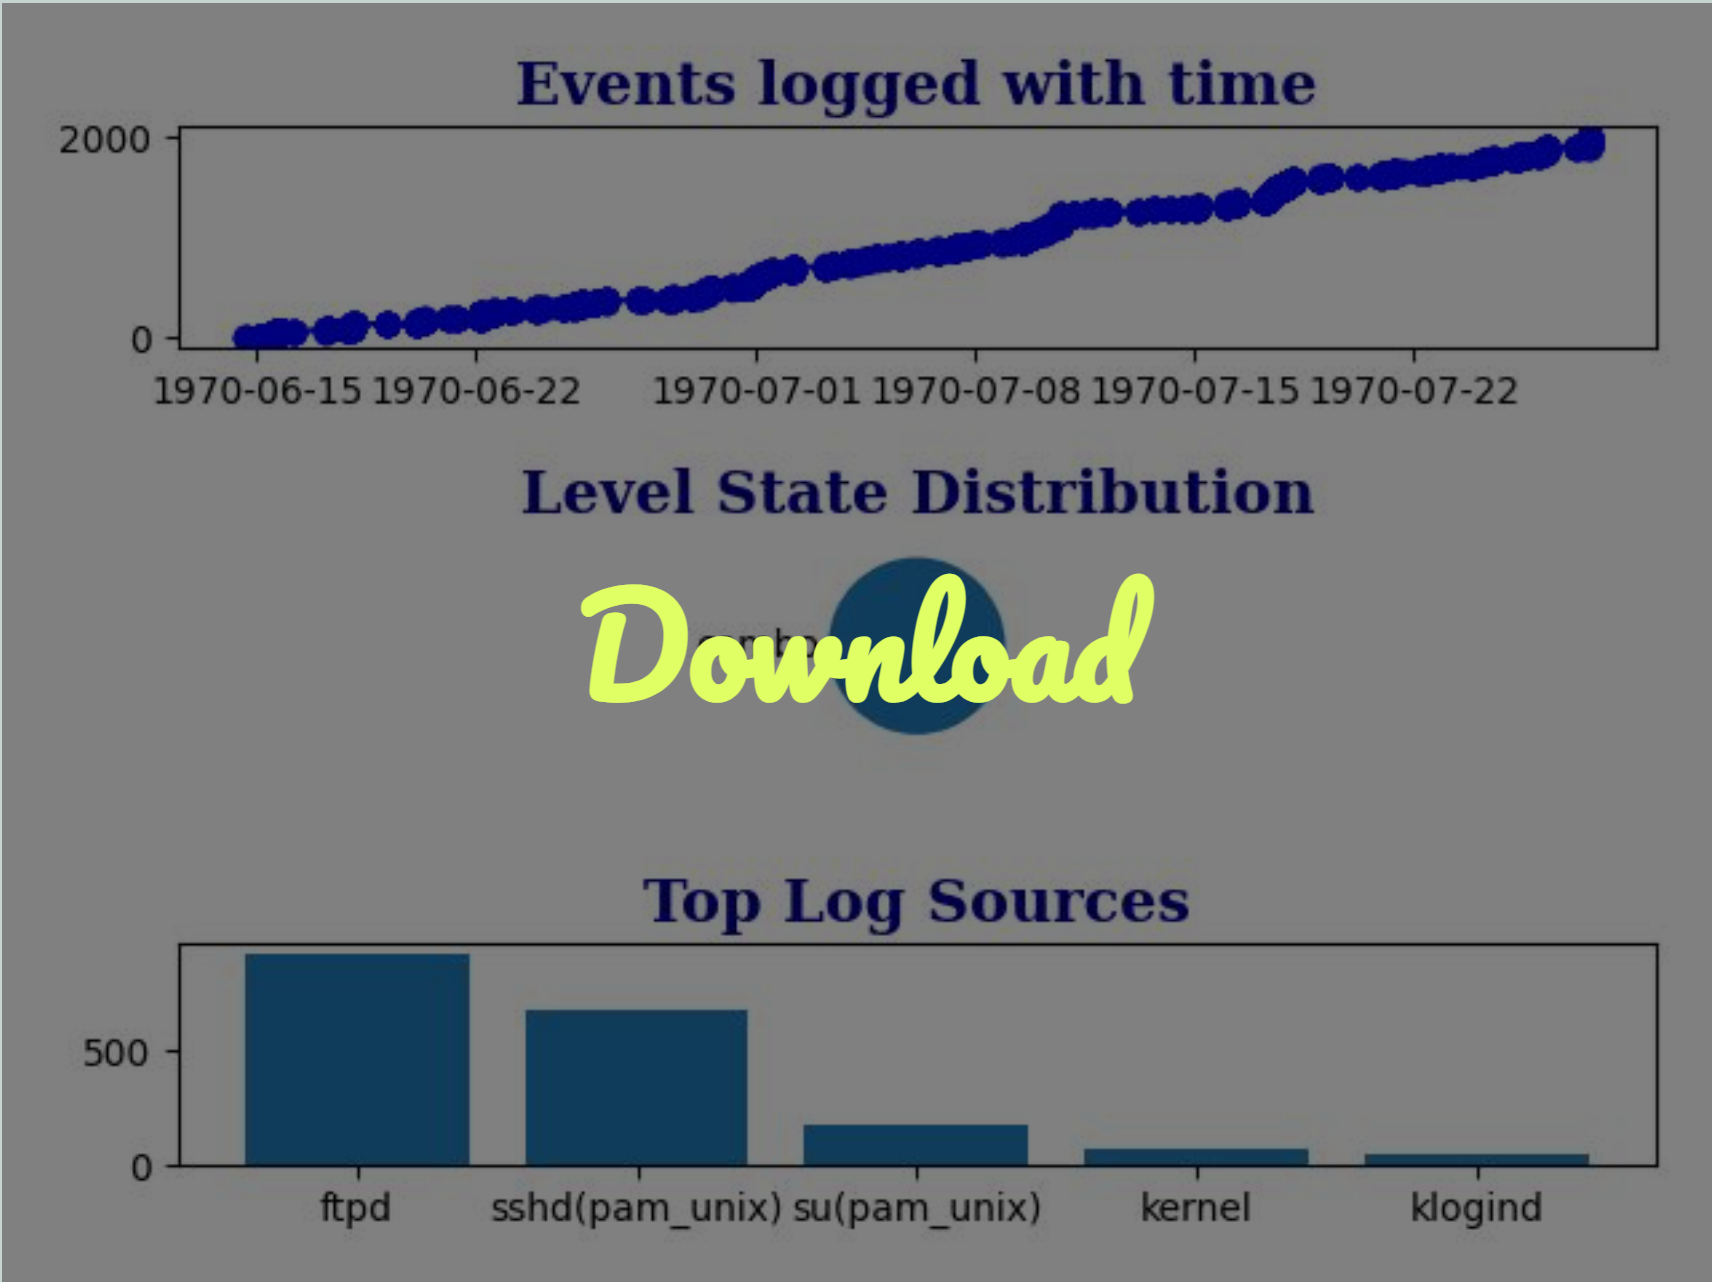
\includegraphics[width=0.8\linewidth]{images/downloadplot.png}
  \caption{On hovering at the displayed plot in the plotting graph page, there
  is an option to download the plot.}
  \label{downloadplot}

\end{figure}



\section{Website Layout}

\subsection{Philosophy}
\label{philo}

\begin{enumerate} 
  \item \textbf{Lazy execution:} This bypasses the need for a
  scheduler if the user uploads multiple files that need to be processed and
  reduces the burden on the server. While it is easy (and perhaps more natural)
  to automate some of these things, this design allowed for easier debugging and
  decent performance on my PC (much less powerful than a server).

  \item \textbf{Use simple webpage elements:} The only thing that I am
  importing from an external source is the caligraphic font for the status
  displayed at the bottom of the webpages. There are no imported libraries for 
  HTML/CSS/JS because I wanted to only use things that I can understand as basic
  features of HTML/CSS/JS themselves rather than relying on ``magic'' done by
  somebody else.

  \item \textbf{Consistent Interface:} All constituent webpages share as much
    HTML/CSS as possible; I have tried to make the functioning of the website
    clear and easy to remember and use (since bash scripts are the slowest part
    of the server-side, if the user explicitly clicks the buttons starting the
    bash scripts, then they will have some idea as to why it is taking time to
    load).
\end{enumerate}

\subsection{The Webpages}

The website consists of four webpages, namely,

\begin{enumerate}
  \item \textbf{Main Page:} Gives a short introduction to the website and a mini
    usage guide. I felt that the first page being an uploads page might feel out
    of context. It is possible to compress the pages together but as per project
    guidelines \cite{logfileprob}, we needed at least three webpages.
  \item \textbf{Upload Files:} Allows the user to upload files. Currently
    supported formats are shown in the drop down menu (Apache log files,
    Android log files and Linux Syslog). By default, it auto
    detects the log type and informs the user of any failure.
  \item \textbf{Show Tables:} Makes structured csv and displays interactive
    tables; also allows the download of csvs filtered by \texttt{from} and
    \texttt{to} dates.
  \item \textbf{Show Plots:} Plots the data in structured csv
    files over custom date ranges. The image can be downloaded in both
    \texttt{png} and \texttt{jpeg} formats by clicking on the displayed plot on
    the website (by default no download is started).
\end{enumerate}

\subsection{Implemented Features}
\label{features}

Although the features were introduced alongside the discussion, here is a
short summary.

\begin{enumerate}
  \item \textbf{General:} There is a title bar, navbar and a status bar
    (depending on the function of the webpage) on each of the four webpages --
    \texttt{main, upload, table, plot}.
  \item \textbf{Uploads:} 
  \begin{itemize}
  \item Auto-detection of log file type (manual selection also supported), 
  \item Drag-and-drop interface for uploading files (dialog box also supported),
  \item A status bar indicating the health of uploaded log files
    \begin{itemize}
    \item displays valid or invalid log file
    \item type of log file detected and shown
    \item declared invalid if detected and input types different
    \item shows time of upload of file
    \item multiple uploads allowed in same app instance (one by one)
    \end{itemize}
  \end{itemize}
  \item \textbf{Table:} 
  \begin{itemize}
    \item Production of structured csv on demand independent of
    order of upload, 
    \item Displays table of the requested processed log file,
    \item Only completely processed files appear in the ``Show
      Table'' drop-down list
      \begin{itemize}
        \item invalid log files are automatically eliminated from further
          processing
        \item tables from any of the uploaded files can be displayed
      \end{itemize}
    \item Interactive displayed tables,
    \begin{itemize}
      \item clicking on a heading sorts by that in ascending order and every
        next click toggles the order of sorting
      \item a unicode arrow shows the order of sorting of the last
        clicked column
      \item this arrow is removed if a heading other than the last one is clicked
      \item clicking on a data cell only displays rows whose entry in the column
        of the clicked element is same as the clicked element itself
      \item clicking on a data cell twice restores the rest of the table
    \end{itemize}
    \item A status bar informing about all unprocessed valid log files,
    \item Download of table from a start date to an end date
    \begin{itemize}
      \item if a start or end date is not provided, then it is ignored in the
        sorting
      \item default behaviour is to download the entire table
    \end{itemize}

    \end{itemize}
  \item \textbf{Plots:}
  \begin{itemize}
    \item Shows plot of the selected log from a start date to an end date
    \begin{itemize}
      \item same behaviour as the sorting options implemented in table page
    \end{itemize}
    \item Hovering over the displayed plot hints the user of a download option
    \item Clicking on the image takes the user to an image endpoint for downloads
  \end{itemize}

\end{enumerate}


\newpage 

\section{Internals}
\label{section:internals}

\subsection{External Dependencies}

\begin{itemize}
  \item The \textit{Pacifio cursive} font taken from
    \href{https://fonts.googleapis.com/css2?family=Pacifico&display=swap}{Google APIs}.

  \item Here is a simplified view of external python
    dependencies\footnote{However, observe that different modules are imported
    in different files.}:
    \begin{verbatim}
      import numpy as np
      import os, csv, subprocess
      import matplotlib.pyplot as plt
      from datetime import datetime
      from flask import Flask, render_template
      from flask import request, send_file, send_directory
      from werkzeug.utils import secure_filename
    \end{verbatim}

    \texttt{np.datetime64} was useful for plotting with \texttt{matplotlib}.  The
    \texttt{os} module provides \texttt{os.path.join} and \texttt{os.makedirs}
    while the \texttt{subprocess} module calls relevant bash scripts. To
    display the table for files containing \texttt{,} and \texttt{""} in their
    fields\footnote{Making use of some complex but widely acknowledged csv
    standards.}, \texttt{csv} module was used (since support for these file
    formats is treated as a part of customization). The \texttt{datetime}
    library is used to keep a track of upload time of the file and nothing else.
    Finally, there is import of some flask utility functions and a standard
    security import \texttt{werkzeug.utils.secure\_filename} (which
    tries to eliminate Javascript injection attacks in file names).

\end{itemize}

\subsection{Directory Structure}
The project uses three different tools: \texttt{bash}, \texttt{python}, and web
development tools. We also have this {\LaTeX} report. The folders that
correspond to each of these things are as follows:

\begin{enumerate}
  \item \textbf{Bash:} The \texttt{Validator} directory contains bash scripts
    for validation of Apache log files as well as Android and Syslog (Linux)
    files. Similarly, the scripts for producing structured csv is in
    \texttt{Parser} while those that filter the csv by date are in
    \texttt{Filter}.

  \item \textbf{Python:} The kick-starting file named
    \texttt{flaskwebsite\_24b0913.py} lies at the root of the project. All other
    python files lie inside the \texttt{app} folder.

  \item \textbf{Web Tools:} All the HTML pages written using
    \texttt{Jinja2} templating engine lie in the \texttt{templates} directory.
    Javascript files are in \texttt{static/js} while all the CSS lies in the
    file \texttt{static/style.css}.

\item \textbf{{\LaTeX} report:} Just for completeness, I added a \texttt{Report}
    directory that contains this report and an \texttt{images} folder inside
    that stores all figures.
\end{enumerate}

\begin{figure}[htbp]

  \centering
  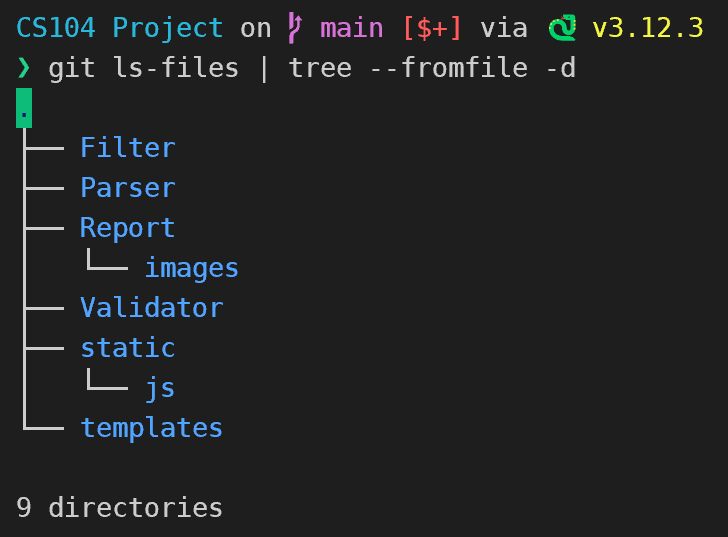
\includegraphics{images/directory.png}
  \caption{An overview of the directory structure.}
  \label{directory}

\end{figure}

Note that there are three more directories that are only formed temporarily,
namely \texttt{uploads, csv, img}. These contain the files uploaded by the user,
the structured csvs after processing and the plot images respectively.
Now we shall see what all files each of these folders contain.

\begin{itemize}
  \item \texttt{Validator:} This contains the files named
    \texttt{*\_validator.sh}.
  \item \texttt{Parser:} The main scripts have names of the form
    \texttt{log\_parser\_*.sh}. Event templates have been manually converted to
    regexes and stored in files named \texttt{*.txt} and \texttt{*.csv}.
    Finally, there are some associated \texttt{awk} scripts with questionable
    file names (for example, \texttt{main.awk} is only used for Android
    logs\footnote{To be fair, it is possible to use it in other log parsers but
    they all have their own regex files in different formats and revamping is
    quite doable but the work has been already done.}). They were emotionally
    named based on the thinking process I had followed.
  \item \texttt{Filter:} This contains organized files with names
    \texttt{*\_filter.sh} and \texttt{*\_filter.awk} because the ugly work has
    been done during parsing.
  \item \texttt{static/js:} The files are named based on their purpose, e.g.,
    \texttt{table\_click.js} handles the click events in the displayed table
    that allow for dynamic sorting and filtering using Javascript.
  \item \texttt{templates:} The \texttt{layout.html} file is the backbone of the
    website design and contains all the dreaded HTML boilerplate. Each
    webpage also has its own file.
  \item \texttt{app:} This folder contains the following files:
    \begin{itemize}
      \item \texttt{config.py:} It contains the global dictionary tracking
        uploaded files and some metadata. Some auxillary variables like
        \texttt{SUPPORTED\_LOG\_FORMATS} and \texttt{*\_TIME\_LADDER} act
        as conveniences. Folders used for validations, parsing, filtering,
        uploading files, etc have their names stored in this file.
      \item \texttt{routes.py:} This contains the logic for handling requests
        made by the client and all the \texttt{@app.routes}. It imports
        functions providing a high-level interface from \texttt{*utils.py}.
      \item \texttt{utils.py:} This contains my implementation of
        \texttt{Counter.most\_common} as we were not allowed to import that
        module. \texttt{find\_*\_date} functions are useful for casting the
        input received from forms into a compact format that can be given to a
        bash script. These functions could not be grouped into other files.
      \item \texttt{pathutils.py:} The site is designed to keep files processed
        to a certain extent in the same location. Keeping this in mind,
        functions in this file do the ugly formatting work and path joining.
      \item \texttt{*utils.py:} I have tried to keep function names fairly
        intuitive, so there should not be much issue with the semantics. One
        thing that deserves special mention is the \texttt{plt.close()} line in
        \texttt{plotutils.py}. It turns out that without this line, there is an
        issue with the flask application which is unable to return to the main
        loop (because of intereference from \texttt{matplotlib}). I learnt this
        the hard way \texttt{;)}

    \end{itemize}
\end{itemize}

\newpage

\section{Project Journey}
Throughout this project, I learnt a variety of new things. Let us go topic-wise.

\subsection{Bash -- Awk and Sed}

The heart of the log processing are the bash scripts. More precisely,
\texttt{awk} scripts (\texttt{sed} was mostly used for sanitization against ugly
\textbackslash\texttt{r} and in general is less powerful to process arrays of regex).
The builtin \texttt{awk} functions had to be used extensively and this activity
gave me an exposure of how to use them. 

One of the hardest thing was to
debugging the regexes that I had written using event templates. The way the
\texttt{awk} regex engine parses is different for variables and raw
strings so I was there in escaping and quotation hell. 

Earlier I learnt to debug by using the excel skills that we had learnt in class
and sorting the columns in various ways depending on lines that were missing.
When it would come to absolute fine tuning though, I had to resort to the
\texttt{diff} command to compare my output with the sample structured csv.

Debugging meant running some \texttt{diff} commands and grepping the appropriate
lines and the regexes and looking at them until it clicked. Many times it was
just a weird case that I had not seen before. For instance, in some fields some
name was ending with a colon while others were not (and the sample's fields did
not contain colons -- they were junk to be eliminated\footnote{One of the cases
where choosing the appropriate \texttt{awk} function was especially helpful.}).

This project yet again showed me the inportance of reading documentation from
official sources like \cite{gawk-builtin-functions} for \texttt{awk} functions
because they are most reliable and mostly to the point (although it is true that
some of them like the bash manual are not the most friendly ones to read even
though they contain all what you need).




\subsection{Python -- Flask and Jinja2}

I had never used a framework like \texttt{Flask} to build a website. Thus, I
referred to tutorials like \cite{flasktutorial} and
\cite{learnflaskfreecodecamp} along with the official website \cite{flaskdocs}.
Initially all of my code was in a single file named
\texttt{flaskwebsite\_24b0913.py}, but as the project began to grow I decided to
split it into multiple files. It was mostly clear how to split because my code
was structured roughly like this:

\begin{verbatim}
  @app.route(`/path/to/page')
  def name_of_route():

  if condition:
    do something
    call_function()
    ...

  return render_template(...)

  def call_function(args):
    ...
\end{verbatim}

Therefore, the main body went into \texttt{app/routes.py} while the associated
functions were put in \texttt{*utils.py}. Before the refactoring I thought that
I knew how the applciation worked. I did not. The errors during refactoring
taught me how the application worked (first I searched online sources and asked
ChatGPT that why the \texttt{Jinja2} templating engine was unable to detect my
HTML templates when they were present in the default directory and that it was fine
before I had tried refactoring).

Essentially, the idea is that the \texttt{Flask(\_\_name\_\_)} that produces the
current app instance should be present at the root of the project (made
in \texttt{flaskwebsite\_24b0913.py} for me). Then you may import your
routes from whichever files you have in \texttt{app/}. However, these have to
import the app instance from \emph{the file that produced the app instance} and
\emph{not} \texttt{flask}.

As a side not, I also got to know that \texttt{Jinja2} is used in contexts outside of
Flask and developing websites -- for templating network device configurations
and database replication.

\subsection{Javascript -- File Event Handling}

Haha, the crazy dialect. I thought that I could get away without using
Javascript in this project at all (so strongly believing in my mistaken
thoughts that they became partial motivation to do this project; in retrospect,
the initial impulse of avoiding Javascript was stereotype-driven but now it is
experience-driven), but as I tried to add more customization to the website, I
understood why it was actually required. 

For example, I wanted to do the table filtering-on-click customization but I was
unable to figure out how do I send python this table that is being made using a
\texttt{Jinja2} template. Eventually I understood that instead of reloading the
entire webpage anytime you clicked, it makes more sense to do this on the
client-side using Javascript.

As another example, in the plotting webpage I want the user to download the plot
and also see the plot. If I try to code both at server-side using the same
button then what will the server respond with? Should it send a file or a newly
rendered webpage? Such self questioning helped me to gain a better understanding
of how the web works. Ultimately I felt that making two buttons was too ugly so
I added a feature where clicking the image sents you to the download route for
the image file (thanks to Javascript).

I realized that I did not understand and know many of the object attributes that
were needed to complete my tasks. Just for completeness, I will detail the basic
principles behind all three of my Javascript files. It was truly fascinating to
know that what I know as ``click to download'', for example, was something
completely else.

\begin{itemize}
  \item \texttt{start\_plot\_download.js:} You first find the plot image on the
    webpage using \texttt{querySelector} and create a link element. The target
    of this link was set using \texttt{link.href = plot.src}. Finally to detect
    clicks, you add an event listener which does a weird thing: it creates the
    hypothetical object as a part of the document, \emph{clicks} it, and
    \emph{then deletes} it (the flashy effects are done using CSS and have
    nothing to do with Javascript at all \dots not quite click to
    download\footnote{it \emph{is} click to download but the semantics is
    different})!
  \item \texttt{drag\_and\_drop.js:} You make a \texttt{div} that constitutes
    the drag-and-drop zone. Then you add an event handler that checks whether
    the user has dragged a file into that zone (and highlight it using CSS).
    Apparently there is a \texttt{dataTransfer.files} attribute that event
    objects have that allows them to ``catch the file to be sent to the
    server''. More precisely, it is a \texttt{FileList}, which is like an
    array of files that were dropped. Input fields of type \texttt{file} have a
    \texttt{files} attribute that allows them to keep track of which files where
    uploaded (these are updated as necesssary).
  \item \texttt{table\_click.js:} This was a bit hard to do. I tried to write an
    implementation which failed without giving errors (even in the browser
    console) so I had to take substantial amount of help from the internet.
    There are two event listeners: one listening for clicks on headings of the
    table and the other listening to clicks on the data cells. They make use of
    some special attributes of objects that I did not know. Conceptually, it
    checks the value of the cell nearest to user click and acts appropriately
    depending on the internal state.

\end{itemize}

Finally comes our honorable mention: \textbf{Git}. This was the first time I used
git for a relatively large project involving thousands of lines of codes. It
gave me a sense of progress with a touch of smugness since I had worked hard to
remember and understand the usage of various git commands. I felt greater
confidence while adding new features because of this additional security. For
documentation purposes, I explicitly note that WSL's git was used so that line
endings remain \textbackslash\texttt{n} and so not interefere if the app has to
run on Unix based systems.

\section{Conclusion}

It was a long and meaningful journey to making my first Flask application and a
challenging experience to write the necessary shell scripts for the job. I
learnt how to use \texttt{flask}, \texttt{Jinja2} templates, structure web
applications (which was mostly done based intuition) and organize my
\texttt{python} code. Javascript is a powerful but spooky language.

\newpage
\bibliographystyle{alpha}
\bibliography{references.bib}

\end{document}
